% Created by tikzDevice version 0.12.6 on 2026-03-25 10:56:36
% !TEX encoding = UTF-8 Unicode
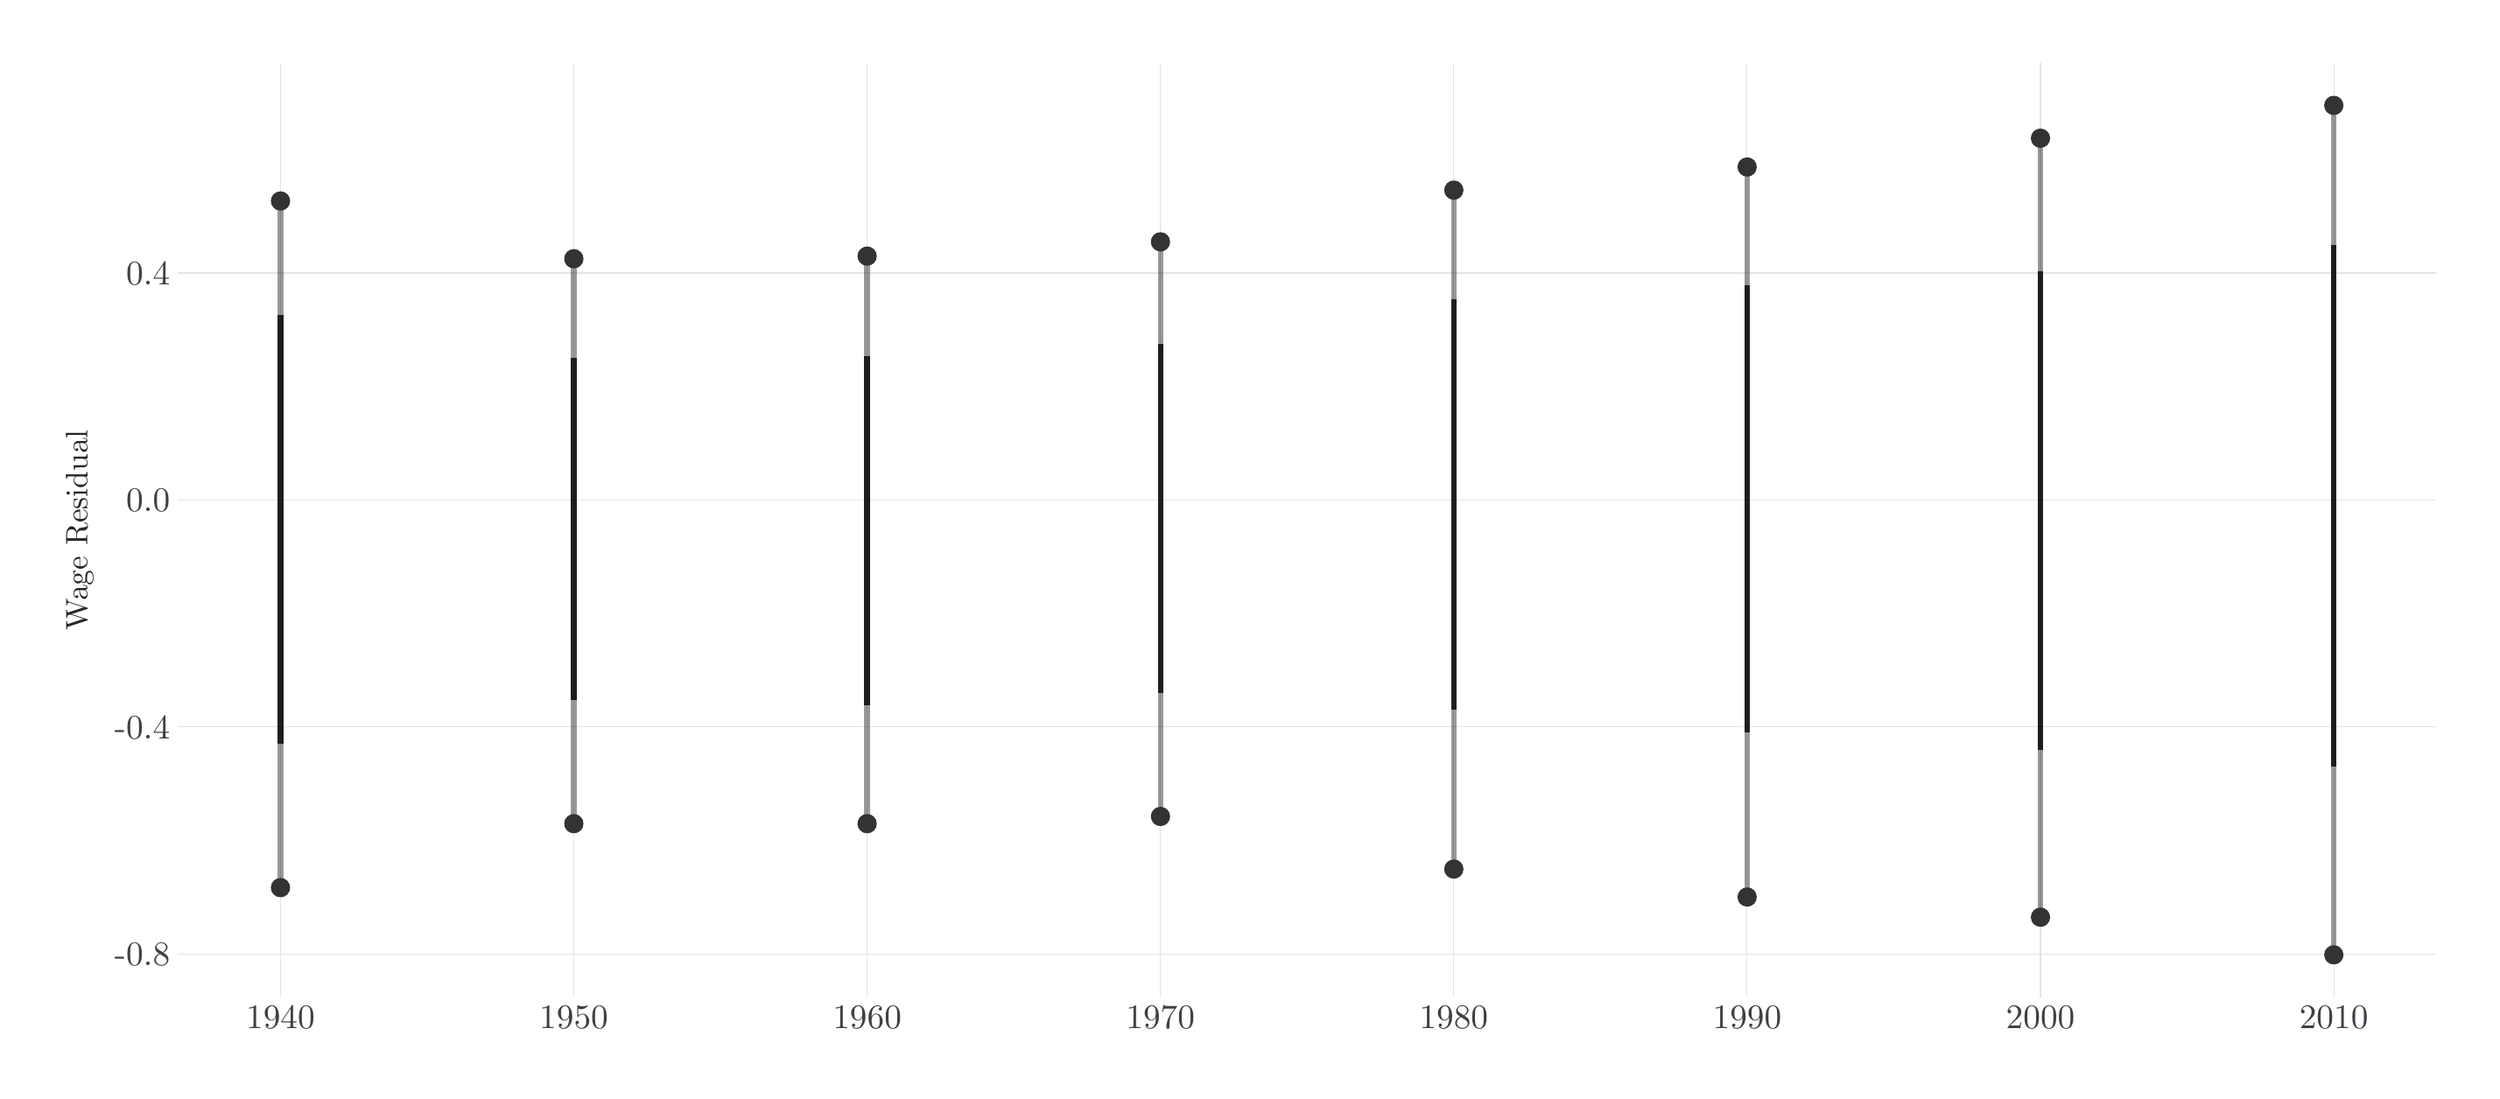
\begin{tikzpicture}[x=1pt,y=1pt]
\definecolor{fillColor}{RGB}{255,255,255}
\path[use as bounding box,fill=fillColor] (0,0) rectangle (1011.78,433.62);
\begin{scope}
\path[clip] (  0.00,  0.00) rectangle (1011.78,433.62);
\definecolor{drawColor}{RGB}{255,255,255}

\path[draw=drawColor,line width= 0.8pt,line join=round,line cap=round,fill=fillColor] (  0.00,  0.00) rectangle (1011.78,433.62);
\end{scope}
\begin{scope}
\path[clip] ( 63.41, 31.76) rectangle (995.78,417.62);
\definecolor{drawColor}{RGB}{255,255,255}
\definecolor{fillColor}{RGB}{255,255,255}

\path[draw=drawColor,line width= 0.8pt,line join=round,line cap=round,fill=fillColor] ( 63.41, 31.76) rectangle (995.78,417.62);
\definecolor{drawColor}{RGB}{228,228,231}

\path[draw=drawColor,line width= 0.4pt,line join=round] ( 63.41, 49.64) --
	(995.78, 49.64);

\path[draw=drawColor,line width= 0.4pt,line join=round] ( 63.41,143.39) --
	(995.78,143.39);

\path[draw=drawColor,line width= 0.4pt,line join=round] ( 63.41,237.14) --
	(995.78,237.14);

\path[draw=drawColor,line width= 0.4pt,line join=round] ( 63.41,330.89) --
	(995.78,330.89);

\path[draw=drawColor,line width= 0.4pt,line join=round] (105.79, 31.76) --
	(105.79,417.62);

\path[draw=drawColor,line width= 0.4pt,line join=round] (226.88, 31.76) --
	(226.88,417.62);

\path[draw=drawColor,line width= 0.4pt,line join=round] (347.96, 31.76) --
	(347.96,417.62);

\path[draw=drawColor,line width= 0.4pt,line join=round] (469.05, 31.76) --
	(469.05,417.62);

\path[draw=drawColor,line width= 0.4pt,line join=round] (590.14, 31.76) --
	(590.14,417.62);

\path[draw=drawColor,line width= 0.4pt,line join=round] (711.22, 31.76) --
	(711.22,417.62);

\path[draw=drawColor,line width= 0.4pt,line join=round] (832.31, 31.76) --
	(832.31,417.62);

\path[draw=drawColor,line width= 0.4pt,line join=round] (953.40, 31.76) --
	(953.40,417.62);
\definecolor{drawColor}{RGB}{0,0,0}

\path[draw=drawColor,draw opacity=0.40,line width= 2.3pt,line join=round] (105.79, 77.05) -- (105.79,360.61);

\path[draw=drawColor,draw opacity=0.40,line width= 2.3pt,line join=round] (226.88,103.47) -- (226.88,336.76);

\path[draw=drawColor,draw opacity=0.40,line width= 2.3pt,line join=round] (347.96,103.47) -- (347.96,337.85);

\path[draw=drawColor,draw opacity=0.40,line width= 2.3pt,line join=round] (469.05,106.45) -- (469.05,343.74);

\path[draw=drawColor,draw opacity=0.40,line width= 2.3pt,line join=round] (590.14, 84.72) -- (590.14,365.10);

\path[draw=drawColor,draw opacity=0.40,line width= 2.3pt,line join=round] (711.22, 73.18) -- (711.22,374.65);

\path[draw=drawColor,draw opacity=0.40,line width= 2.3pt,line join=round] (832.31, 64.84) -- (832.31,386.54);

\path[draw=drawColor,draw opacity=0.40,line width= 2.3pt,line join=round] (953.40, 49.30) -- (953.40,400.08);
\definecolor{drawColor}{RGB}{0,0,0}

\path[draw=drawColor,draw opacity=0.80,line width= 2.3pt,line join=round] (105.79,136.33) -- (105.79,313.51);

\path[draw=drawColor,draw opacity=0.80,line width= 2.3pt,line join=round] (226.88,154.49) -- (226.88,295.99);

\path[draw=drawColor,draw opacity=0.80,line width= 2.3pt,line join=round] (347.96,152.44) -- (347.96,296.44);

\path[draw=drawColor,draw opacity=0.80,line width= 2.3pt,line join=round] (469.05,157.55) -- (469.05,301.76);

\path[draw=drawColor,draw opacity=0.80,line width= 2.3pt,line join=round] (590.14,150.55) -- (590.14,320.21);

\path[draw=drawColor,draw opacity=0.80,line width= 2.3pt,line join=round] (711.22,141.04) -- (711.22,325.69);

\path[draw=drawColor,draw opacity=0.80,line width= 2.3pt,line join=round] (832.31,133.87) -- (832.31,331.66);

\path[draw=drawColor,draw opacity=0.80,line width= 2.3pt,line join=round] (953.40,127.16) -- (953.40,342.29);
\definecolor{drawColor}{gray}{0.20}
\definecolor{fillColor}{gray}{0.20}

\path[draw=drawColor,line width= 0.5pt,line join=round,line cap=round,fill=fillColor] (105.79, 77.05) circle (  3.73);

\path[draw=drawColor,line width= 0.5pt,line join=round,line cap=round,fill=fillColor] (226.88,103.47) circle (  3.73);

\path[draw=drawColor,line width= 0.5pt,line join=round,line cap=round,fill=fillColor] (347.96,103.47) circle (  3.73);

\path[draw=drawColor,line width= 0.5pt,line join=round,line cap=round,fill=fillColor] (469.05,106.45) circle (  3.73);

\path[draw=drawColor,line width= 0.5pt,line join=round,line cap=round,fill=fillColor] (590.14, 84.72) circle (  3.73);

\path[draw=drawColor,line width= 0.5pt,line join=round,line cap=round,fill=fillColor] (711.22, 73.18) circle (  3.73);

\path[draw=drawColor,line width= 0.5pt,line join=round,line cap=round,fill=fillColor] (832.31, 64.84) circle (  3.73);

\path[draw=drawColor,line width= 0.5pt,line join=round,line cap=round,fill=fillColor] (953.40, 49.30) circle (  3.73);

\path[draw=drawColor,line width= 0.5pt,line join=round,line cap=round,fill=fillColor] (105.79,360.61) circle (  3.73);

\path[draw=drawColor,line width= 0.5pt,line join=round,line cap=round,fill=fillColor] (226.88,336.76) circle (  3.73);

\path[draw=drawColor,line width= 0.5pt,line join=round,line cap=round,fill=fillColor] (347.96,337.85) circle (  3.73);

\path[draw=drawColor,line width= 0.5pt,line join=round,line cap=round,fill=fillColor] (469.05,343.74) circle (  3.73);

\path[draw=drawColor,line width= 0.5pt,line join=round,line cap=round,fill=fillColor] (590.14,365.10) circle (  3.73);

\path[draw=drawColor,line width= 0.5pt,line join=round,line cap=round,fill=fillColor] (711.22,374.65) circle (  3.73);

\path[draw=drawColor,line width= 0.5pt,line join=round,line cap=round,fill=fillColor] (832.31,386.54) circle (  3.73);

\path[draw=drawColor,line width= 0.5pt,line join=round,line cap=round,fill=fillColor] (953.40,400.08) circle (  3.73);
\end{scope}
\begin{scope}
\path[clip] (  0.00,  0.00) rectangle (1011.78,433.62);
\definecolor{drawColor}{RGB}{63,63,70}

\node[text=drawColor,anchor=base east,inner sep=0pt, outer sep=0pt, scale=  1.42] at ( 60.21, 44.74) {-0.8};

\node[text=drawColor,anchor=base east,inner sep=0pt, outer sep=0pt, scale=  1.42] at ( 60.21,138.49) {-0.4};

\node[text=drawColor,anchor=base east,inner sep=0pt, outer sep=0pt, scale=  1.42] at ( 60.21,232.24) {0.0};

\node[text=drawColor,anchor=base east,inner sep=0pt, outer sep=0pt, scale=  1.42] at ( 60.21,325.99) {0.4};
\end{scope}
\begin{scope}
\path[clip] (  0.00,  0.00) rectangle (1011.78,433.62);
\definecolor{drawColor}{RGB}{63,63,70}

\node[text=drawColor,anchor=base,inner sep=0pt, outer sep=0pt, scale=  1.42] at (105.79, 18.76) {1940};

\node[text=drawColor,anchor=base,inner sep=0pt, outer sep=0pt, scale=  1.42] at (226.88, 18.76) {1950};

\node[text=drawColor,anchor=base,inner sep=0pt, outer sep=0pt, scale=  1.42] at (347.96, 18.76) {1960};

\node[text=drawColor,anchor=base,inner sep=0pt, outer sep=0pt, scale=  1.42] at (469.05, 18.76) {1970};

\node[text=drawColor,anchor=base,inner sep=0pt, outer sep=0pt, scale=  1.42] at (590.14, 18.76) {1980};

\node[text=drawColor,anchor=base,inner sep=0pt, outer sep=0pt, scale=  1.42] at (711.22, 18.76) {1990};

\node[text=drawColor,anchor=base,inner sep=0pt, outer sep=0pt, scale=  1.42] at (832.31, 18.76) {2000};

\node[text=drawColor,anchor=base,inner sep=0pt, outer sep=0pt, scale=  1.42] at (953.40, 18.76) {2010};
\end{scope}
\begin{scope}
\path[clip] (  0.00,  0.00) rectangle (1011.78,433.62);
\definecolor{drawColor}{RGB}{39,39,42}

\node[text=drawColor,rotate= 90.00,anchor=base,inner sep=0pt, outer sep=0pt, scale=  1.28] at ( 26.06,224.69) {Wage Residual};
\end{scope}
\end{tikzpicture}
